\begin{figure}[htbp]
\centering
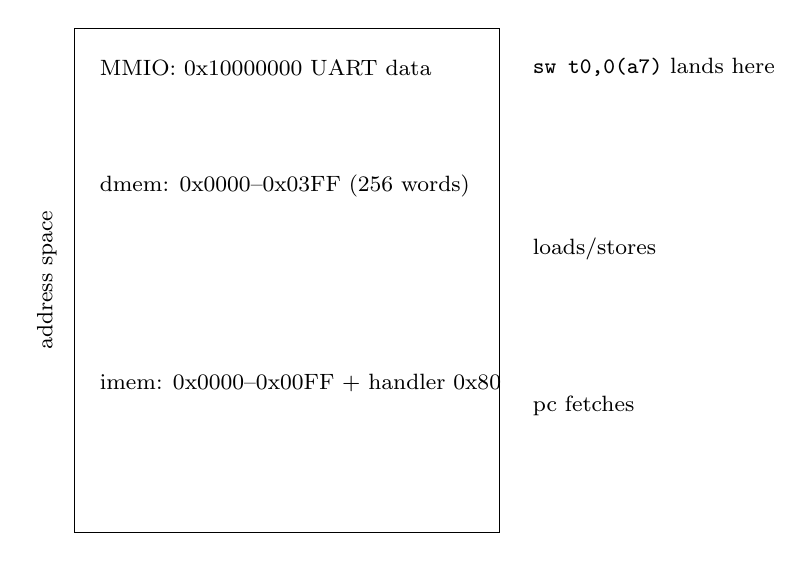
\begin{tikzpicture}[font=\footnotesize]
  \draw (0,0) rectangle (5.4,6.4);
  \foreach \y/\h/\lbl/\fill in
    {5.4/1.0/MMIO: 0x10000000 UART data/red!14,
     3.4/2.0/dmem: 0x0000--0x03FF (256 words)/blue!10,
     0.4/3.0/imem: 0x0000--0x00FF + handler 0x80/green!12} {
    \fill[\fill] (0.1,\y) rectangle (5.3,\y+\h);
    \node[anchor=west] at (0.2,\y+\h/2) {\lbl};
  }
  \node[rotate=90, anchor=center] at (-0.35,3.2) {address space};
  \node[anchor=west] at (5.7,5.9) {\texttt{sw t0,0(a7)} lands here};
  \node[anchor=west] at (5.7,3.6) {loads/stores};
  \node[anchor=west] at (5.7,1.6) {pc fetches};
\end{tikzpicture}
\caption{The flat address map seen by ch08 programs. Instruction
fetch lives low, data loads/stores in the middle, and one carved-out
address --- 0x10000000 --- belongs to the UART.}
\label{fig:mmio08}
\end{figure}
